% ============================================================================
%  Chapitre 4, partie III : Algorithme de simulation en quaternions
% ============================================================================

% ----------------------------------------------------------------------------
\section{Algorithme de simulation - Orientation en quaternions}
% ----------------------------------------------------------------------------

La simulation en angles d'Euler ne tient que tant que
$|\cos\theta| > \varepsilon$. Dans cette partie, on garde la même
dynamique, mais on représente l'orientation par un quaternion unitaire
pour supprimer cette singularité.

% ----------------------------------------------------------------------------
\subsection{Motivation : problème du gimbal lock}

\subsubsection{Perte d'un degré de liberté}

Les colonnes de $\mat{E}$ donnent la vitesse angulaire produite par
chaque angle :
\[
    \pd{\vect{\omega}}{\dot\varphi} = \begin{pmatrix}
        1\\ 0\\ 0
    \end{pmatrix},
    \qquad
    \pd{\vect{\omega}}{\dot\theta} = \begin{pmatrix}
        0\\ c_\varphi\\ -s_\varphi
    \end{pmatrix},
    \qquad
    \pd{\vect{\omega}}{\dot\psi} = \begin{pmatrix}
        -s_\theta\\ s_\varphi c_\theta\\ c_\varphi c_\theta
    \end{pmatrix}
\]
Lorsque $\theta = \pm\pi/2$, la troisième colonne devient
$(\mp 1, 0, 0)$, colinéaire à la première : $\varphi$ et $\psi$
décrivent la même rotation. On perd un degré de liberté, et
$\det\mat{E} = \cos\theta = 0$.

\subsubsection{Conséquence pour la simulation}

La sphère, elle, peut toujours tourner autour de l'axe bloqué. Mais
pour décrire cette rotation en angles d'Euler, il faut
\[
    \dot\alpha = \mat{E}^{-1}\,\vect{\omega}
\]
dont les composantes sont en $1/\cos\theta$. Près de la singularité,
un petit mouvement selon l'axe bloqué donne donc des vitesses
$\dot\varphi$ et $\dot\psi$ très grandes, et des accélérations
$\ddot\alpha$ plus grandes encore. Le système réduit devient mal
conditionné, et le schéma RK4 à pas fixe perd sa précision. Cependant, le mouvement de la sphère n'a rien de particulier. La singularité vient uniquement de la représentation de l'orientation, pas de la physique. Il suffit donc de changer la représentation de l'orientation d'où la solution avec les quaternions.

\subsubsection{Solution par les quaternions}

Un quaternion unitaire $\quat{q}$ décrit l'orientation avec $4$
paramètres liés par $\|\quat{q}\| = 1$. La matrice de rotation
$\mat{R}(\quat{q})$ et la cinématique $\dot{\quat{q}} = \tfrac12\,\quat{q}\quatmul(0,\vect{\omega})$ sont définies pour toute orientation et il n'y a plus de
singularité. Le prix à payer est un paramètre redondant, et une
renormalisation de $\quat{q}$ au cours de la simulation, qui ne sont pas trop chers par rapport à la stabilité que l'on va gagner.

% ----------------------------------------------------------------------------
\subsection{Dynamique du système en représentation quaternionique}

\subsubsection{État}

\textbf{Quaternion des angles d'Euler : } Avec la définition de représentation quaternionique d'une rotation $\theta$ autour d'un axe unitaire $\vect{u}$ du chapitre 2, et avec la convention
$Z$-$Y'$-$X''$, le quaternion est
le produit des trois rotations élémentaires, dans le même ordre que
$\mat{R} = \mat{R}_z(\psi)\,\mat{R}_y(\theta)\,\mat{R}_x(\varphi)$ :
\[
    \quat{q}(\alpha)
    = \Bigl(\cos\tfrac{\psi}{2},\, 0,\, 0,\, \sin\tfrac{\psi}{2}\Bigr)
    \quatmul\Bigl(\cos\tfrac{\theta}{2},\, 0,\, \sin\tfrac{\theta}{2},\, 0\Bigr)
    \quatmul\Bigl(\cos\tfrac{\varphi}{2},\, \sin\tfrac{\varphi}{2},\, 0,\, 0\Bigr)
\]

On décrit l'orientation par $\quat{q}$ et la rotation par la vitesse
angulaire $\vect{\omega}$ exprimée dans le corps. L'état est ainsi 
\[
    Y = (\quat{q},\vect{\omega})\in\R^7, \quad \text{avec} \quad \|\quat{q}\| = 1
\]
soit $7$ nombres pour $6$ degrés de liberté. Comme démontré plus haut avec les angles d'Euler, on peut calculer la position à part. On cherche donc seulement à écrire
\[
    \dot Y = \begin{pmatrix}
        \dot{\quat{q}}\\ \dot{\vect{\omega}}
    \end{pmatrix}
    = \begin{pmatrix}
        \tfrac12\,\quat{q}\quatmul(0,\vect{\omega})\\
        \dot{\vect{\omega}}
    \end{pmatrix}
\]
La première composante est la cinématique quaternionique. Il nous reste à trouver l'équation de $\dot{\vect{\omega}}$.

\subsubsection{Équation de \texorpdfstring{$\dot{\vect{\omega}}$}{omega point}}
Il suffit ici d'utiliser les équations de Gibbs-Appell avec $\vect{\omega}$ comme
pseudo-vitesses.
D'abord, il nous faut retrouver la fonction de Gibbs-Appell en fonction de $\vect{\omega}$.
Soit $\vect{\gamma}$ l'axe vertical vu depuis le corps, $\vect{\gamma}$ s'écrit ainsi dans le repère corps :
\[
    \vect{\gamma} = \mat{R}(\quat{q})^T\vect{e}_z
\]
D'après la fonction de Gibbs-Appell d'un solide, à des termes sans $\dot{\vect{\omega}}$ près, on a :
\[
    \mathcal{G} = \frac{1}{2}\,m\,\|\vect{a}_G\|^2
    + \frac{1}{2}\,\dot{\vect{\omega}}^T\mat{I}_b\,\dot{\vect{\omega}}
    + \dot{\vect{\omega}}\cdot\bigl(\vect{\omega}\wedge
    \mat{I}_b\vect{\omega}\bigr)
\]
On voit que le seul terme qu'il reste à calculer est $\vect{a}_G$.

\textbf{Dérivées de $\mat{R}$ et $\vect{\gamma}$ : } Comme
$\vect{\Omega} = \mat{R}\,\vect{\omega}$,
\[
    \dot{\mat{R}} = \hatx{\vect{\Omega}}\,\mat{R}
    = \mat{R}\,\hatx{\vect{\omega}}
\]
et comme $\vect{e}_z$ est fixe,
\[
    \dot{\vect{\gamma}} = \dot{\mat{R}}^T\vect{e}_z
    = -\,\hatx{\vect{\omega}}\,\mat{R}^T\vect{e}_z
    = -\,\vect{\omega}\wedge\vect{\gamma}
    = \vect{\gamma}\wedge\vect{\omega}
\]

\textbf{Accélération du centre : } D'après le roulement, avec
$\vect{\Omega} = \mat{R}\,\vect{\omega}$ et
$\vect{e}_z = \mat{R}\,\vect{\gamma}$, on a :
\[
    \vect{v}_G = a\,\vect{\Omega}\wedge\vect{e}_z
    = a\,\mat{R}\vect{\omega}\wedge\mat{R}\vect{\gamma}
\]
puis, comme une rotation conserve le produit vectoriel,
\[
    \vect{v}_G = a\,\mat{R}\,(\vect{\omega}\wedge\vect{\gamma})
\]
En dérivant ce terme, on a l'accélération :
\[
    \vect{a}_G = a\,\mat{R}\Bigl(
    \vect{\omega}\wedge(\vect{\omega}\wedge\vect{\gamma})
    + \dot{\vect{\omega}}\wedge\vect{\gamma}
    + \vect{\omega}\wedge(\vect{\gamma}\wedge\vect{\omega})\Bigr)
\]
Le premier et le dernier terme s'annulent, car
$\vect{\omega}\wedge\vect{\gamma} + \vect{\gamma}\wedge\vect{\omega}
= \vect{0}$, d'où
\[
    \vect{a}_G = a\,\mat{R}\,(\dot{\vect{\omega}}\wedge\vect{\gamma})
\]
Comme $\mat{R}$ conserve la norme,
$\|\vect{a}_G\| = a\,\|\dot{\vect{\omega}}\wedge\vect{\gamma}\|$.

\begin{proposition}[Fonction de Gibbs-Appell de la sphère avec $\vect{\omega}$ comme pseudo-vitesse]
    Avec $\vect{\omega}$ comme pseudo-vitesse, la fonction de
    Gibbs-Appell de la sphère s'écrit :
    \[
        \mathcal{G} = \tfrac12\,m\,a^2\,
        \|\dot{\vect{\omega}}\wedge\vect{\gamma}\|^2
        + \tfrac12\,\dot{\vect{\omega}}^T\mat{I}_b\,\dot{\vect{\omega}}
        + \dot{\vect{\omega}}\cdot(\vect{\omega}\wedge\mat{I}_b\,
        \vect{\omega})
    \]
\end{proposition}
Ensuite, on développe le premier terme en utilisant la formule de la
norme d'un produit vectoriel
$\|\vect{u}\wedge\vect{v}\|^2 = \|\vect{u}\|^2\,\|\vect{v}\|^2
- (\vect{u}\cdot\vect{v})^2$ avec $\|\vect{\gamma}\| = 1$ :
\[
    \|\dot{\vect{\omega}}\wedge\vect{\gamma}\|^2
    = \|\dot{\vect{\omega}}\|^2
    - (\dot{\vect{\omega}}\cdot\vect{\gamma})^2
    = \dot{\vect{\omega}}^T\bigl(\Id - \vect{\gamma}\vect{\gamma}^T
    \bigr)\dot{\vect{\omega}}
\]
On réécrit la fonction de Gibbs-Appell sous la forme :
\[
    \mathcal{G} = \tfrac12\,\dot{\vect{\omega}}^T\mat{K}(\vect{\gamma})
    \,\dot{\vect{\omega}}
    + \dot{\vect{\omega}}\cdot(\vect{\omega}\wedge\mat{I}_b\,
    \vect{\omega}) \quad \text{avec} \quad
    \mat{K}(\vect{\gamma}) = \mat{I}_b
    + m\,a^2\,\bigl(\Id - \vect{\gamma}\vect{\gamma}^T\bigr)
\]
Le potentiel $V = m g a$ est constant et aucune force non
conservative n'est appliquée, donc $\mathcal{Q} = 0$. On en déduit
l'équation de Gibbs-Appell :
\[
    \pd{\mathcal{G}}{\dot{\vect{\omega}}}
    = \mat{K}(\vect{\gamma})\,\dot{\vect{\omega}}
    + \vect{\omega}\wedge\mat{I}_b\,\vect{\omega} = \vect{0}
\]
\begin{proposition}[Inversibilité de $\mat{K}(\vect{\gamma})$]
    La matrice $\mat{K}(\vect{\gamma})$ est symétrique, définie positive donc inversible.
\end{proposition}
\begin{demonstration}
    On voit bien que $\mat{K}(\vect{\gamma})$ est symétrique,
    et pour tout $\vect{v}\neq\vect{0}$,
    \[
        \vect{v}^T\mat{K}(\vect{\gamma})\,\vect{v}
        = \vect{v}^T\mat{I}_b\,\vect{v}
        + m\,a^2\,\|\vect{v}\wedge\vect{\gamma}\|^2
        \geq \vect{v}^T\mat{I}_b\,\vect{v} > 0
    \]
    car $\mat{I}_b$ est définie positive. $\mat{K}$ est donc inversible.
\end{demonstration}

\begin{proposition}[Dynamique en quaternions]
    Avec
    \[
        \mat{K}(\vect{\gamma}) = \mat{I}_b
        + m\,a^2\,\bigl(\Id - \vect{\gamma}\vect{\gamma}^T\bigr)
    \]
    on a
    \[
        \mat{K}(\vect{\gamma})\,\dot{\vect{\omega}}
        = -\,\vect{\omega}\wedge\mat{I}_b\,\vect{\omega}
    \]
\end{proposition}

On a donc la dynamique
\[
    \dot Y = f(Y)= \begin{pmatrix}
        \tfrac12\,\quat{q}\quatmul(0,\vect{\omega})\\
        -\,\mat{K}(\vect{\gamma})^{-1}
        \bigl(\vect{\omega}\wedge\mat{I}_b\,\vect{\omega}\bigr)
    \end{pmatrix}
\]
définie pour toute orientation, sans condition sur $\cos\theta$.

\subsubsection{Position et frottements}

Une fois $Y$ connu, la position et les frottements s'en déduisent sans
nouvelle équation. On repasse dans le repère du sol avec
$\vect{\Omega} = \mat{R}\,\vect{\omega}$. On a, avec
$\dot{\mat{R}} = \mat{R}\,\hatx{\vect{\omega}}$,
\[
    \dot{\vect{\Omega}} = \mat{R}\,(\vect{\omega}\wedge\vect{\omega})
    + \mat{R}\,\dot{\vect{\omega}}
    = \mat{R}\,\dot{\vect{\omega}}
\]

\textbf{Position : }
\[
    \dot{\vect{r}} = \vect{v}_G = \begin{pmatrix}
        \dot x\\ \dot y\\ 0
    \end{pmatrix}
    = a\,\vect{\Omega}\wedge\vect{e}_z
    = a\begin{pmatrix}
        \Omega_y\\ -\,\Omega_x\\ 0
    \end{pmatrix}
\]
On peut simplement calculer $\vect{r}$ avec une quadrature. 

\textbf{Frottements : } D'après la loi de Newton en $x$ et $y$,
$(N_x, N_y, 0) = m\,\vect{a}_G$. Avec
$\vect{a}_G = a\,\mat{R}\,(\dot{\vect{\omega}}\wedge\vect{\gamma})$ et
$\mat{R}\,\vect{\gamma} = \vect{e}_z$ : 
\[
    \vect{a}_G = a\,\dot{\vect{\Omega}}\wedge\vect{e}_z
    = a\begin{pmatrix}
        \dot\Omega_y\\ -\,\dot\Omega_x\\ 0
    \end{pmatrix}
\]

\begin{proposition}[Position et frottements]
    Avec $\vect{\Omega} = \mat{R}(\quat{q})\,\vect{\omega}$ et
    $\dot{\vect{\Omega}} = \mat{R}(\quat{q})\,\dot{\vect{\omega}}$,
    \[
        \dot x = a\,\Omega_y,
        \qquad
        \dot y = -\,a\,\Omega_x,
        \qquad
        N_x = m\,a\,\dot\Omega_y,
        \qquad
        N_y = -\,m\,a\,\dot\Omega_x
    \]
    et $N_z = m g$. Le non-glissement se vérifie a posteriori par
    \[
        \sqrt{N_x^2 + N_y^2} \leq \mu_s\,m\,g
    \]
\end{proposition}

% ----------------------------------------------------------------------------
\subsection{Schéma numérique}

On reprend le schéma RK4 de la partie II pour $\dot Y = f(Y)$, mais
cette fois-ci $Y = (\quat{q},\vect{\omega})$. La seule nouveauté est la
renormalisation de $\quat{q}$ à chaque pas.

\subsubsection{Conditions initiales}

\begin{proposition}[Conditions initiales]
    Les conditions initiales de cette dynamique sont
    $(r_0, \quat{q}(0), \vect{\omega}_0)$.
\end{proposition}

Comme en partie II, on se donne la position $r_0$, l'orientation
$\alpha_0$ et la vitesse angulaire $\vect{\Omega}_0$ dans $\rep{s}$.
On en déduit
\[
    \quat{q}(0) = \quat{q}(\alpha_0),
    \qquad
    \vect{\omega}_0 = \mat{R}\bigl(\quat{q}(0)\bigr)^T\vect{\Omega}_0
\]
Contrairement aux angles d'Euler, il n'y a aucune condition sur
$\cos\theta_0$ : on n'inverse plus $\mat{E}_s$. Enfin,
$\dot{\vect{\omega}}_0$ et les frottements initiaux s'obtiennent en
faisant les mêmes calculs que les étapes 3 et 4.

\subsubsection{Choix du pas}

\subsubsection{Schéma RK4 pour simuler le système}

\paragraph{Étape 1 : Orientation} Avec
$Y_k = (\quat{q}_k,\vect{\omega}_k)$, on évalue $f$ en quatre états
intermédiaires du pas,
\[
    Y^{(1)} = Y_k,
    \qquad
    Y^{(2)} = Y_k + \tfrac{h}{2}\,\vect{p}_1,
    \qquad
    Y^{(3)} = Y_k + \tfrac{h}{2}\,\vect{p}_2,
    \qquad
    Y^{(4)} = Y_k + h\,\vect{p}_3
\]
où $Y^{(i)} = (\quat{q}^{(i)},\vect{\omega}^{(i)})$ et
\[
    \vect{p}_i = f\bigl(Y^{(i)}\bigr)
    = \begin{pmatrix}
        \dot{\quat{q}}^{(i)}\\ \dot{\vect{\omega}}^{(i)}
    \end{pmatrix},
    \qquad
    \dot{\quat{q}}^{(i)} = \tfrac12\,\quat{q}^{(i)}\quatmul
    (0,\vect{\omega}^{(i)})
\]
avec
\[
    \mat{K}\bigl(\vect{\gamma}^{(i)}\bigr)\,\dot{\vect{\omega}}^{(i)}
    = -\,\vect{\omega}^{(i)}\wedge\mat{I}_b\,\vect{\omega}^{(i)},
    \qquad
    \vect{\gamma}^{(i)} = \mat{R}\bigl(\quat{q}^{(i)}\bigr)^T\vect{e}_z
\]
On obtient alors le nouvel état :
\[
    \quat{q}_{k+1} = \quat{q}_k + \tfrac{h}{6}\,\bigl(\dot{\quat{q}}^{(1)}
    + 2\,\dot{\quat{q}}^{(2)} + 2\,\dot{\quat{q}}^{(3)}
    + \dot{\quat{q}}^{(4)}\bigr),
    \qquad
    \vect{\omega}_{k+1} = \vect{\omega}_k + \tfrac{h}{6}\,\bigl(
    \dot{\vect{\omega}}^{(1)} + 2\,\dot{\vect{\omega}}^{(2)}
    + 2\,\dot{\vect{\omega}}^{(3)} + \dot{\vect{\omega}}^{(4)}\bigr)
\]

\paragraph{Étape 2 : Renormalisation} La dynamique conserve
$\|\quat{q}\| = 1$, mais pas le schéma : l'erreur est en
$O(h^5)$ sur un pas et s'accumule au cours de la simulation. Il nous faut alors 
renormaliser à chaque pas : 
\[
    \quat{q}_{k+1} \longleftarrow
    \frac{\quat{q}_{k+1}}{\|\quat{q}_{k+1}\|}
\]
L'écart $\bigl|\,\|\quat{q}_{k+1}\| - 1\,\bigr|$ avant renormalisation
reste de l'ordre de l'erreur du schéma.

\paragraph{Étape 3 : Accélération} On résout l'équation de
$\dot{\vect{\omega}}$ au nouvel état :
\[
    \mat{K}(\vect{\gamma}_{k+1})\,\dot{\vect{\omega}}_{k+1}
    = -\,\vect{\omega}_{k+1}\wedge\mat{I}_b\,\vect{\omega}_{k+1},
    \qquad
    \vect{\gamma}_{k+1} = \mat{R}(\quat{q}_{k+1})^T\vect{e}_z
\]
C'est la seconde moitié de $f(Y_{k+1})$, réutilisée comme
$\vect{p}_1$ au pas suivant.

\paragraph{Étape 4 : Position et frottements} En parallèle avec
l'étape 1, on calcule des poids RK4 pour $r$ avec
$\vect{g}_i = a\,\bigl(\Omega_y^{(i)}, -\,\Omega_x^{(i)}\bigr)$ et
$\vect{\Omega}^{(i)} = \mat{R}\bigl(\quat{q}^{(i)}\bigr)\,
\vect{\omega}^{(i)}$, tels que :
\[
    r_{k+1} = r_k + \tfrac{h}{6}\,\bigl(\vect{g}_1 + 2\,\vect{g}_2
    + 2\,\vect{g}_3 + \vect{g}_4\bigr)
\]
puis, avec $\dot{\vect{\Omega}}_{k+1} = \mat{R}(\quat{q}_{k+1})\,
\dot{\vect{\omega}}_{k+1}$,
\[
    N_{x,k+1} = m\,a\,\dot\Omega_{y,k+1},
    \qquad
    N_{y,k+1} = -\,m\,a\,\dot\Omega_{x,k+1}
\]

% ----------------------------------------------------------------------------
\subsection{Architecture de la simulation}

Voici l'architecture de la simulation prête à implémenter avec
l'orientation représentée par un quaternion unitaire.

\begin{figure}[H]
    \centering
    \begin{tikzpicture}[>=Stealth,
        bloc/.style={draw, thick, rounded corners=2pt, align=center,
            fill=coulprop!6, draw=coulprop, inner sep=4pt,
            font=\small},
        ctrl/.style={bloc, fill=couldef!8, draw=couldef},
        stop/.style={bloc, fill=coulthm!8, draw=coulthm},
        es/.style={bloc, fill=gray!8, draw=gray},
        fl/.style={->, thick},
        lab/.style={font=\footnotesize, fill=white, inner sep=1pt}]

        \node[es] (in) at (0,0) {Entrées : $m$, $a$, $\mat{I}_b$,
            $\mu_s$ ; $r_0$, $\alpha_0$, $\vect{\Omega}_0$ ; $h$, $N$};
        \node[bloc] (init) at (0,-1.3)
            {Initialisation : $\quat{q}(0) = \quat{q}(\alpha_0)$,
            \quad $\vect{\omega}_0 = \mat{R}\bigl(\quat{q}(0)\bigr)^T
            \vect{\Omega}_0$, \quad
            $Y_0 = \bigl(\quat{q}(0),\vect{\omega}_0\bigr)$};
        \node[bloc] (f) at (0,-3.3)
            {Évaluation de $f$ en $Y^{(i)}$, $i = 1,\dots,4$ :\\[2pt]
            $\dot{\quat{q}}^{(i)} = \tfrac12\,\quat{q}^{(i)}\quatmul
            (0,\vect{\omega}^{(i)})$\\[2pt]
            $\mat{R}\bigl(\quat{q}^{(i)}\bigr)$
            $\;\to\;$ $\vect{\gamma}^{(i)}$
            $\;\to\;$ $\mat{K}\bigl(\vect{\gamma}^{(i)}\bigr)\,
            \dot{\vect{\omega}}^{(i)}
            = -\,\vect{\omega}^{(i)}\wedge\mat{I}_b\,\vect{\omega}^{(i)}$};
        \node[bloc] (rk) at (-2.9,-5.5)
            {Étape 1 : $Y_{k+1}$ par RK4\\[2pt]
            Étape 2 : $\quat{q}_{k+1} \leftarrow
            \quat{q}_{k+1}/\|\quat{q}_{k+1}\|$\\[2pt]
            Étape 3 : $\dot{\vect{\omega}}_{k+1}$};
        \node[bloc] (rl) at (2.9,-5.5)
            {Étape 4 : $r_{k+1}$ avec les $\vect{g}_i$,\\[2pt]
            $N_{x,k+1}$, $N_{y,k+1}$};
        \node[ctrl] (c) at (0,-7.4)
            {Contrôles : $T$, $\vect{L}_P$ conservés ;
            $\sqrt{N_{x,k+1}^2 + N_{y,k+1}^2} \leq \mu_s\,m\,g$};
        \node[stop] (arret) at (-3.6,-9.3)
            {Arrêt : simulation\\non valide};
        \node[es] (out) at (3.6,-9.3)
            {Sorties : $r_k$, $\quat{q}_k$, $\vect{\omega}_k$,
            $(N_x, N_y)_k$,\\
            $k = 0,\dots,N$};

        \draw[fl] (in) -- (init);
        \draw[fl] (init) -- (f);
        \draw[fl] (f) -- (rk);
        \draw[fl] (f) -- (rl);
        \draw[fl] (rk) -- (c);
        \draw[fl] (rl) -- (c);
        \draw[fl, coulthm] (c) -- node[lab, pos=0.45, left=2pt]
            {non} (arret);
        \draw[fl] (c) -- node[lab, pos=0.45, right=2pt]
            {oui, $k = N$} (out);
        \coordinate (droite) at (6.4,0);
        \draw[fl] (c.east) -- (c.east -| droite) -- (f.east -| droite)
            node[lab, pos=0.5, left=2pt, align=right]
            {oui,\\$k \leftarrow k+1$} -- (f.east);

        \begin{scope}[on background layer]
            \node[draw=gray, dashed, rounded corners, inner sep=7pt,
                fit=(f) (rk) (rl) (c) (c.east -| droite)] (boucle) {};
        \end{scope}
        \node[font=\footnotesize, gray, anchor=south west]
            at (boucle.north west) {boucle sur $k$};
    \end{tikzpicture}
    \caption{Architecture de la simulation de la sphère de Chaplygin
    en quaternions}
\end{figure}

Par rapport aux angles d'Euler, le contrôle $|\cos\theta| > \varepsilon$
disparaît, et l'étape de renormalisation s'ajoute.

\subsection{Validation de la simulation}
\subsubsection{Écart avec le modèle en angles d'Euler}

On relance la boule anisotrope de la partie précédente
(figure~\ref{fig-traj-anisotrope}), avec les mêmes paramètres et le même
pas $h$, une fois avec le modèle en angles d'Euler et une fois avec le
modèle en quaternions. Sur ce lancer, $|\cos\theta| \geq 0{,}74$ et les deux modèles décrivent la même
dynamique. Les deux simulations doivent donc donner le même résultat, à l'erreur du schéma près.
\paragraph{Écarts mesurés : } on note avec un indice $E$ (resp. $Q$) les
grandeurs calculées en angles d'Euler (resp. en quaternions), et on
mesure à chaque pas
\[
    \|r_k^E - r_k^Q\|,
    \qquad
    \|\mat{R}_k^E - \mat{R}_k^Q\|_F,
    \qquad
    \|(N_x, N_y)_k^E - (N_x, N_y)_k^Q\|
\]
où $\|\cdot\|_F$ est la norme de Frobenius. Sur les $5$ s de simulation,
ces écarts restent inférieurs à $1{,}1\cdot 10^{-11}$ m,
$2{,}2\cdot 10^{-11}$ et $6{,}7\cdot 10^{-12}$ N respectivement
(figure~\ref{fig-ecart-euler-quat}). La dérive relative de l'énergie
reste de l'ordre de $10^{-12}$ pour les deux modèles.

\begin{figure}[H]
    \centering
    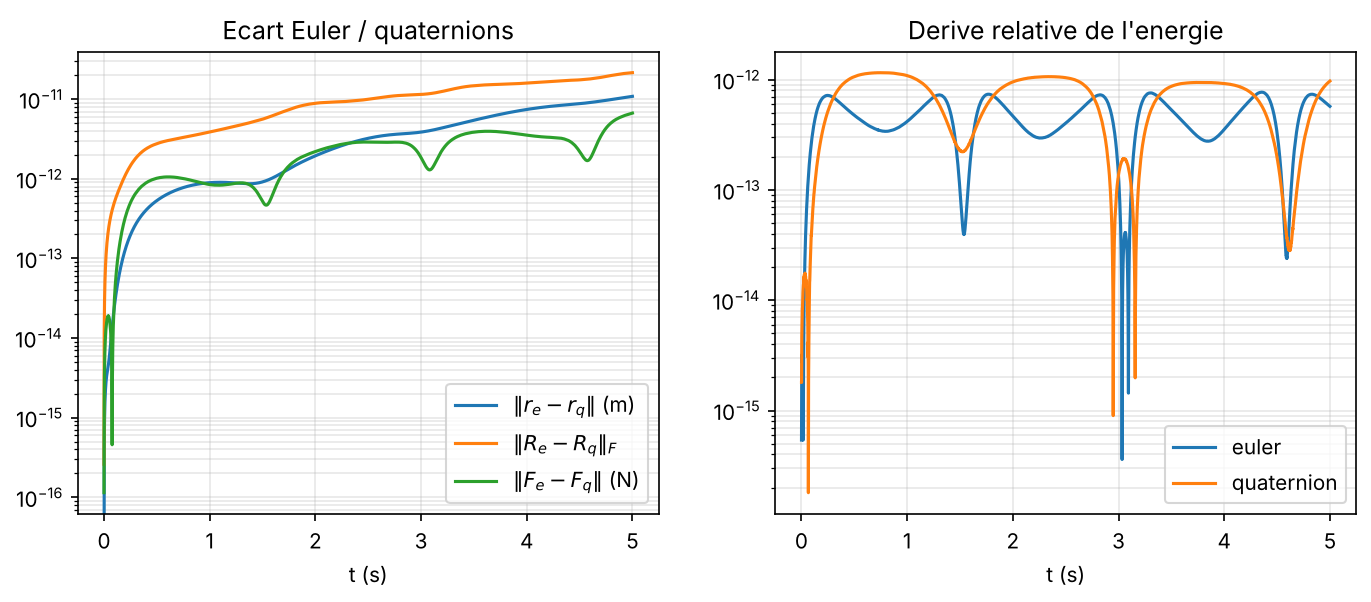
\includegraphics[width=0.95\textwidth]{chapitre4/figures/validation_case_a_errors.png}
    \caption{Boule anisotrope : écart entre les simulations en angles
    d'Euler et en quaternions, et dérive relative de l'énergie}
    \label{fig-ecart-euler-quat}
\end{figure}

Loin de la singularité, la simulation en quaternions redonne donc les
résultats de la simulation en angles d'Euler.

\paragraph{Près du gimbal lock}

On lance maintenant la même boule avec un tangage proche de $90^\circ$ :
\[
    \alpha_0 = (0;\ 90^\circ - 0{,}4^\circ;\ 0),
    \qquad
    \vect{\Omega}_0 = (5;\ 1;\ 2) \text{ rad.s}^{-1}
\]
avec le même pas $h$ et la même durée. On peut par partir de gimbal lock car la simulation en angles d'Euler ne pourrait pas se lancer, mais on peut partir de son voisinage et lui donne de la vitesse pour atteindre gimbal lock.

\textbf{Trajectoire et angles : } les deux simulations coïncident jusqu'à
$t \approx 1{,}84$ s (figure~\ref{fig-gimbal-traj}). Les angles calculés en angles d'Euler s'écartent alors de ceux calculés en quaternions, et la trajectoire de $G$ avec eux :
l'écart atteint $50$ cm à $t = 5$ s.

\begin{figure}[H]
    \centering
    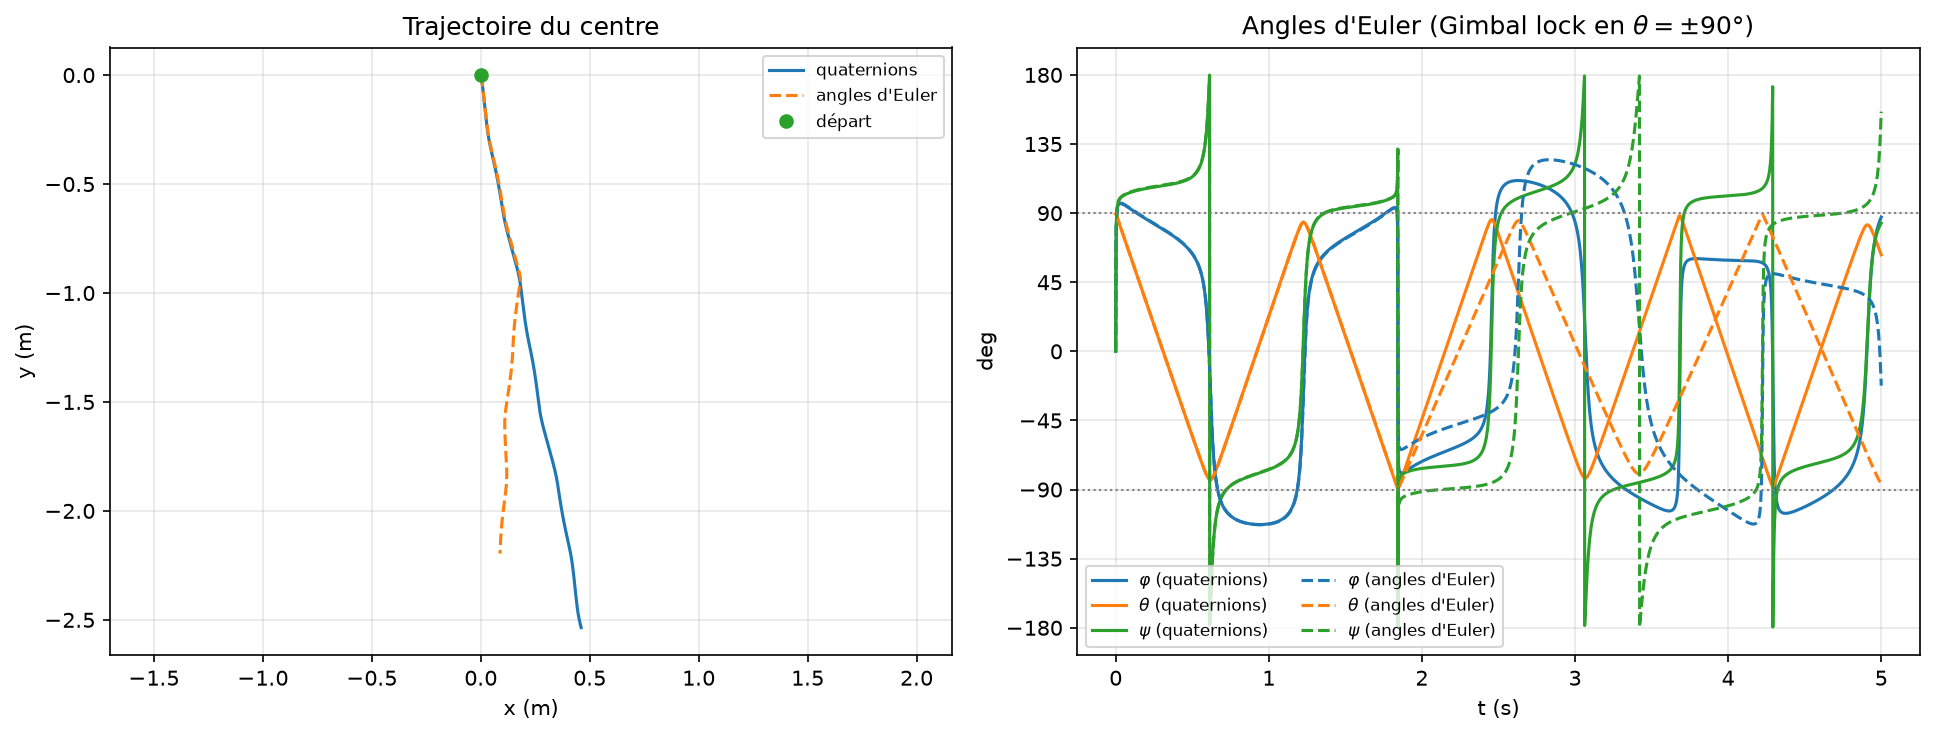
\includegraphics[width=\textwidth]{chapitre4/figures/case_b_euler_vs_quat.png}
    \caption{Près du gimbal lock : trajectoire de $G$ et angles d'Euler,
    calculés en quaternions (trait plein) et en angles d'Euler (tirets)}
    \label{fig-gimbal-traj}
\end{figure}

\textbf{Contrôles : } en quaternions, les dérives relatives de $T$ et de
$\vect{L}_P$ restent de l'ordre de $10^{-12}$
(figure~\ref{fig-gimbal-controles}). En angles d'Euler, les dérives de
$T$ et de $\vect{L}_P$ valent déjà quelques $10^{-3}$ dès le premier pas,
puisqu'on part près de la singularité, puis sautent à $43\ \%$ et
$33\ \%$ au passage de $t \approx 1{,}84$ s. L'erreur du schéma utilisant les angles d'Euler s'accumule dès les premiers pas près de la singularité, donc, pour la trajectoire, ce n'est pas forcément fiable pour la simulation en angles d'Euler.

En revanche, les deux autres contrôles passent : on a toujours
$|\cos\theta| > \varepsilon = 10^{-3}$, et
$\|(N_x, N_y)\| \leq 0{,}47$ N reste loin de $\mu_s\,m\,g \approx 4{,}9$ N.
La simulation en angles d'Euler est donc déclarée valide alors qu'elle
est fausse, on ne peut voir les erreurs qu'à travers les conservations.

\begin{figure}[H]
    \centering
    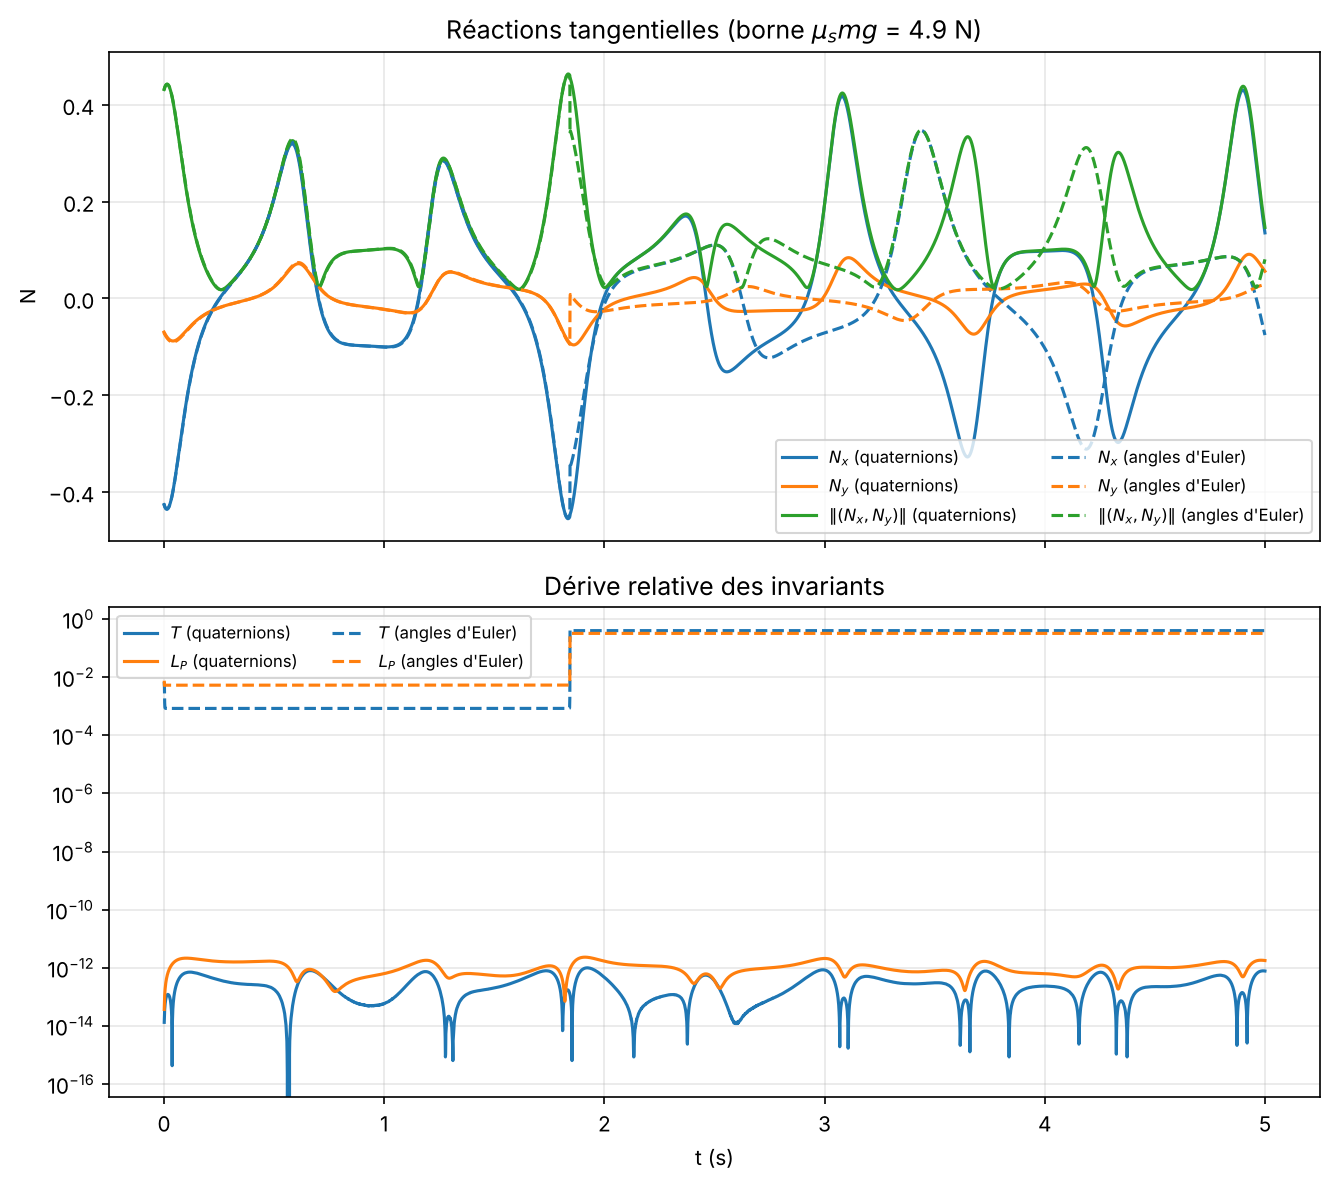
\includegraphics[width=0.8\textwidth]{chapitre4/figures/case_b_controls.png}
    \caption{Près du gimbal lock : réactions tangentielles et dérive
    relative des invariants, en quaternions (trait plein) et en angles
    d'Euler (tirets)}
    \label{fig-gimbal-controles}
\end{figure}

Près de la singularité, seule la simulation en quaternions reste fiable.
